\chapter{Dynamic 3D Object Insertion}\label{chp:ObjectLoading}

In order to realize the insertion of a 3D object from a CAD file, a plug-in with this functionality was developed simply called CADRuntimeImporter(CRI). Alongside it a standalone Unreal prototype project, named CADRuntimePresenter(CRP), was made that incorporates CRI in order to demonstrate how it can be used for a multi-user desktop and VR environment. The whole mechanism can be split into three major sections: opening and parsing the files, generating the objects and lastly user interaction with said objects. How all of that was implemented and what sort of advantages and disadvantages these approaches have, will be discussed in this chapter.
%%%%%%%%%%%%%%%%%%%%%%%%%%%%%%%%%%%%%%%%%%%%%%%%%%%%%%%%%%%%%%%%%%%%%%%%%%%%%%%%%%%%%%%%%%%%%%%%%%%%%%
\section{Loading and Parsing CAD Files}
\subsection{File Loading and Sharing}
The first step in creating an object in runtime is naturally opening the desired file and getting the required data from it in runtime as well. As Unreal Engine is written in C++, it is not surprising that opening up a file isn't too much of an issue. What makes this simpler is the fact that Unreal also offers this in their FileHelper class with the functions LoadFileToString() and LoadFileToArray(). The first function can load a text file into a string, while the other loads binary files into an array of bytes. This is only directly available in C++ and therefore had to be exposed to Blueprints. As this functionality is more of a utility, it isn't the best idea to attach it to a specific object. Luckily for such purposes Unreal offers Blueprint Function Libraries. This is just a special type of Unreal C++ class in which only static functions can be defined. These functions then become available to be used in any Blueprint without needing any instanced objects.\\

Something that is slightly more complicated is actually choosing the file. Here Unreal does technically offer the ability to open a file dialog but this is strictly a developer only module and can't be used in finished products. Even neglecting that, it wouldn't work in VR so a separate solution would have been needed anyway. Due to this a file picker in CRPs UI had to be written. The end result of that can be seen in Figure \ref{fig:FilePicker}. The design is rather simple but offers all the necessary functionality, especially that it is compatible with VR and only displays supported file formats.\\

\begin{figure}[htpb]
	\centering
	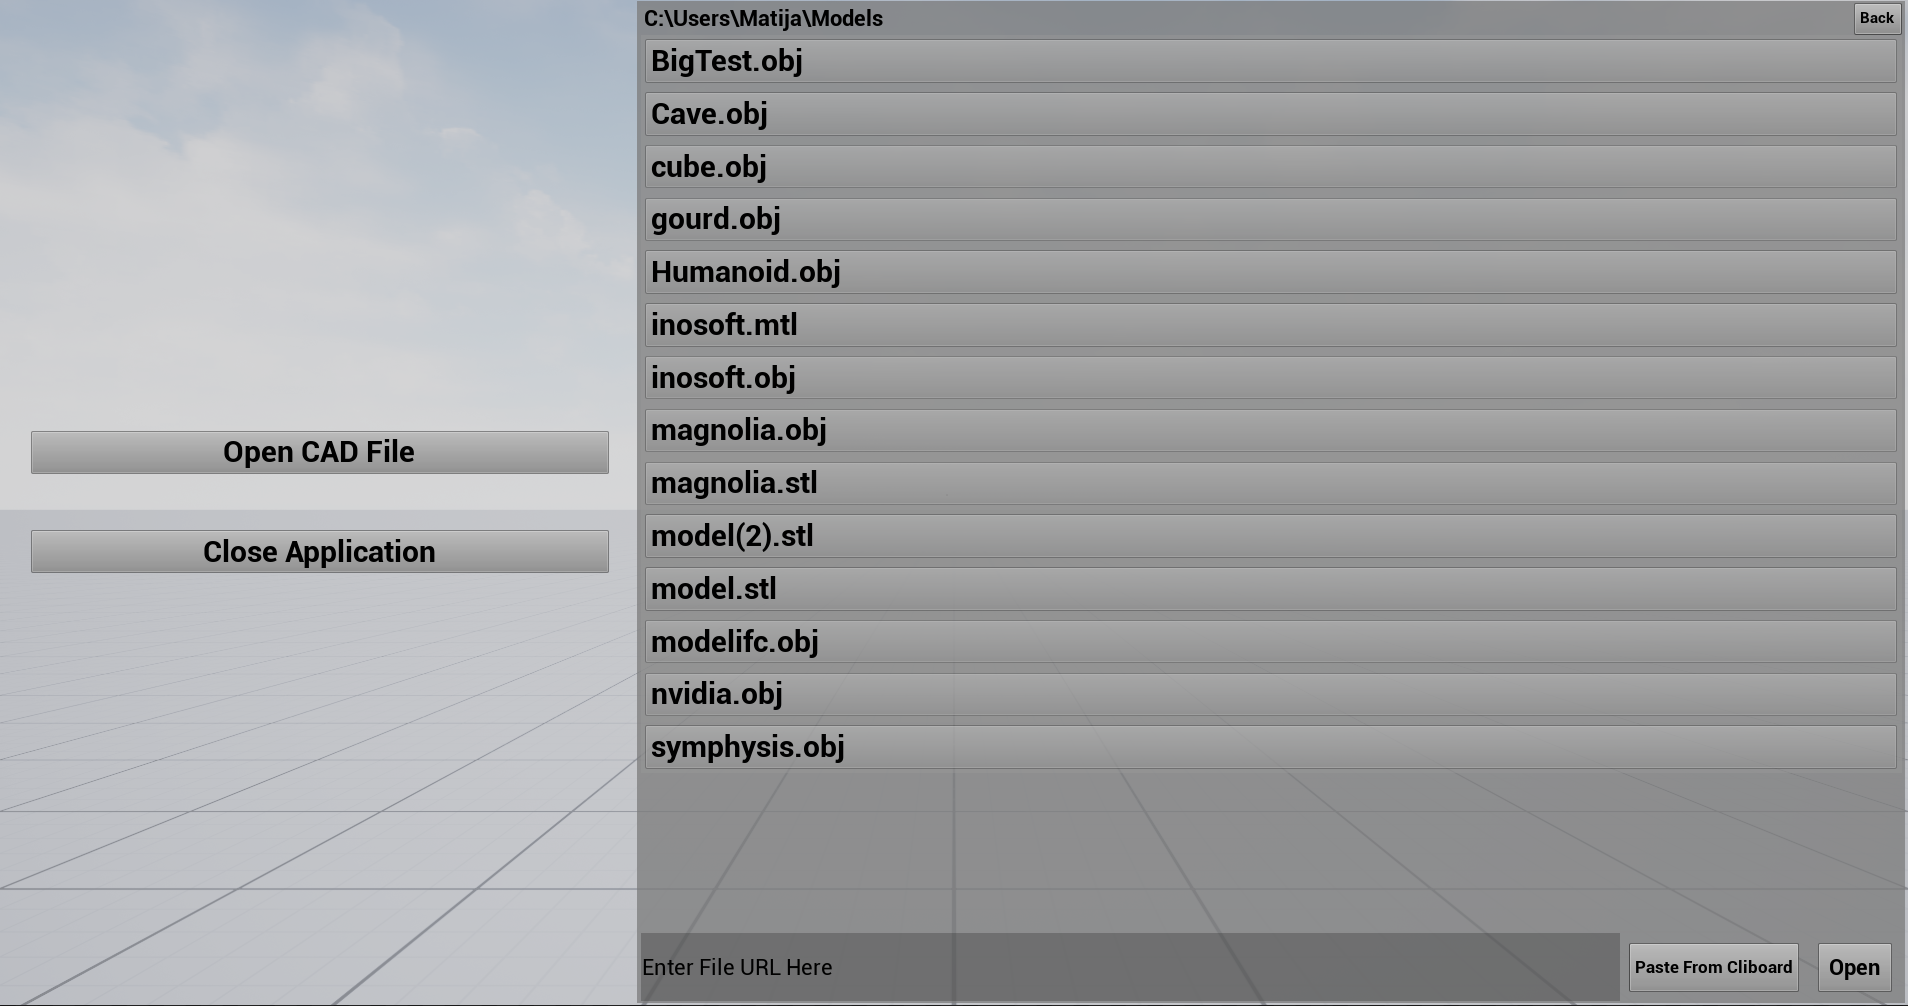
\includegraphics[width=0.9\textwidth]{fig/FilePicker2.png}
	\caption[CAD Runtime Presenter File Picker]{File Picker for CRP\protect}
	\label{fig:FilePicker}
\end{figure}

For a single user this would be enough, they could choose a file and then it could be parsed for object generating. Complications arise once there are multiple users involved. If a user were to open a file in such a scenario, the object would appear only in the world of that user and not for other users or even on the server. This could cause many issues since the clients world would not match servers, which is the authoritative instance. The problem lies in the fact that the new object needs to be created on every client and on the server. In order for that to happen every machine needs access to the required data, not just the client who has the file available on their machine.\\

One way of sharing this data is saving it in a replicated variable and having it handled by the automatic replication. This does actually work but it has one fatal flaw which makes using it not viable. That is the size limit of replicated variables. The size limit for arrays is 64 kilobytes and for strings it seems to about the same. For smaller files this would be a perfect solution but unfortunately CAD files tend to be too big for it.\\
So instead this problem was solved by having the file be uploaded to a server and then be downloaded by the rest of the clients and server. For such purposes Unreal offers the HTTPModule interface, which uses the popular and powerful libcurl library, to create HTTP requests. A file could then be uploaded using a POST request and downloaded using a GET request. For this a simple file server which can handle such requests was written in python. The only problem is that the clients and server need to know where and what file was uploaded in order to make the correct request. This is where replication comes in handy. The client that uploads the file can tell the server where it was uploaded through a replicated string, which is most likely going to be within the size limit, and then the server can propagate that information to the rest of the clients which then make the GET requests.\\
Seeing as for most users only the link to the file matters, this means that the client that wants to open a file doesn't even need to have it locally on their machine. Instead they can simply input a link to a service like Dropbox or Google Drive and have everyone download those files. The UI for that is also part of the file picker and can be seen at the bottom of Figure \ref{fig:FilePicker}.\\
There are technically other libraries and plug-ins that could be used to enable file sharing with more complicated protocols but that wasn't necessary for this prototype project. The HTTPModule is simple to use while offering all the needed functionalities and avoids having to rely too much on third-party libraries.


%%%%%%%%%%%%%%%%%%%%%%%%%%%%%%%%%%%%%%%%%%%%%%%%%%%%%%%%%%%%%%%%%%%%%%%%%%%%%%%%%%%%%%%%%%%%%%%%%%%%%%
\subsection{Parsing Wavefront OBJ and STL}

Once every instance of the program has the desired file, the next step can begin which is parsing the data. What data is available and how it is stored can vary heavily from format to format. Generally they will all have the vertices that define the mesh but outside of that colour, material or anything else isn't guaranteed. This is the case because CAD formats tend to be highly specific for their uses cases, as well as proprietary for the CAD software they were developed for. This makes supporting many CAD formats quite difficult, especially those that aren't well documented or don't even have publicly available documentation. Especially for the scope of this project, spending too much time writing parser for as many formats as possible was not feasible.\\
Instead the decision was made to use well known and widely supported formats, like OBJ and STL. One of the biggest benefits of this approach is the already existing support that these formats have. Many CAD softwares support exporting to one of these and even if they don't, there are probably tools with which the files can be converted. This saved a lot of time in the development, as only a few parsers had to be written and for those that had to be implemented, the process was fairly simple due to all the existing resources on the formats.

\subsubsection{Wavefront OBJ}

Wavefront OBJ, or simply OBJ, is a geometry definition file format developed by Wavefront Technologies for their Advanced Visualizer animation packages. It is a neutral, open source format which has been widely adopted and has good import and export support from almost all CAD software.\\
Another reason why OBJ was chosen is the fact that is can be directly read through any text editor. This helped out a lot in early stages of development where the primary goal was to prove that the concept worked. Being able to see and read the data made it simpler to write a parser in the first place, as well as comprehending what was going on with the data at later stages.\\ 
The format represents 3D geometry in the form of vertex positions, vertex normals, texture coordinates, polygonal faces and groups of faces. These geometries can also use materials indirectly through referencing materials defined in a separate MTL file. Every entry in an OBJ file is represented through a single line, starting with an identifying tag followed by the value of the entry. What these entries can look like is represented in Table \ref{tab:ObjTypes}.

\begin{table}[htbp]
	\centering 
	\scalebox{0.889}{
		\begin{tabular}{lll}
			\toprule \textbf{Tag} & \textbf{Example Value} & \textbf{Definition} \\
			\bottomrule
			v & 0.2 0.3 0.5 & 3D Vector representing 3D Vertex \\
			vn & 1.0 0.5 0.0 & 3D Vector representing 3D Normal \\
			vt & 0.5 0.25 & 2D Vector representing Texture Coordinate\\
			f & 1/1/2  2/2/5  3/3/5 & Polygonal Face made from Vertices, Normals and Textures\\
			usemtl & Stone & Defines what Material should be used for following faces\\
			g & Door & Defines a polygon group\\
			\bottomrule
	\end{tabular}}
	\caption[ObjTypes]{Relevant types in OBJ format}
	\label{tab:ObjTypes}
\end{table}

In order to parse there values, most of the entries can be regarded one-by-one. Vertices, normals and texture coordinates are vectors and can be saved in separate vector arrays in the order in which they appear. How these and the rest of the values are used will be explained later, for now it's only important how they are saved.\\
Faces, materials and group are more complicated as they define how the rest of the data is put together to make the object. A face represents a polygon defined through lists of vertex, texture and normal indices in the format "vertexIndex/textureIndex/normalIndex", as can be seen in Table \ref{tab:ObjTypes}. It is important to note that these are the indices of the values and not the values themselves. Also the indices for vertices, texture coordinates and normals are separate and based on when the entry was defined in the file starting with one. So both a vector and normal can have their respective index be 1. The polygons themselves tend to be triangles but can also have more sides. This isn't ideal as later for generating the mesh only triangles are supported but there is a simple way to solve this. The vertices are listed in a counter clockwise order so that any polygon can be represented through a triangle fan, as is shown in Figure \ref{fig:TriangleFan}. So faces that define polygons with more than 3 edges are replaced through multiple triangles faces.

\begin{figure}[htpb]
	\centering
	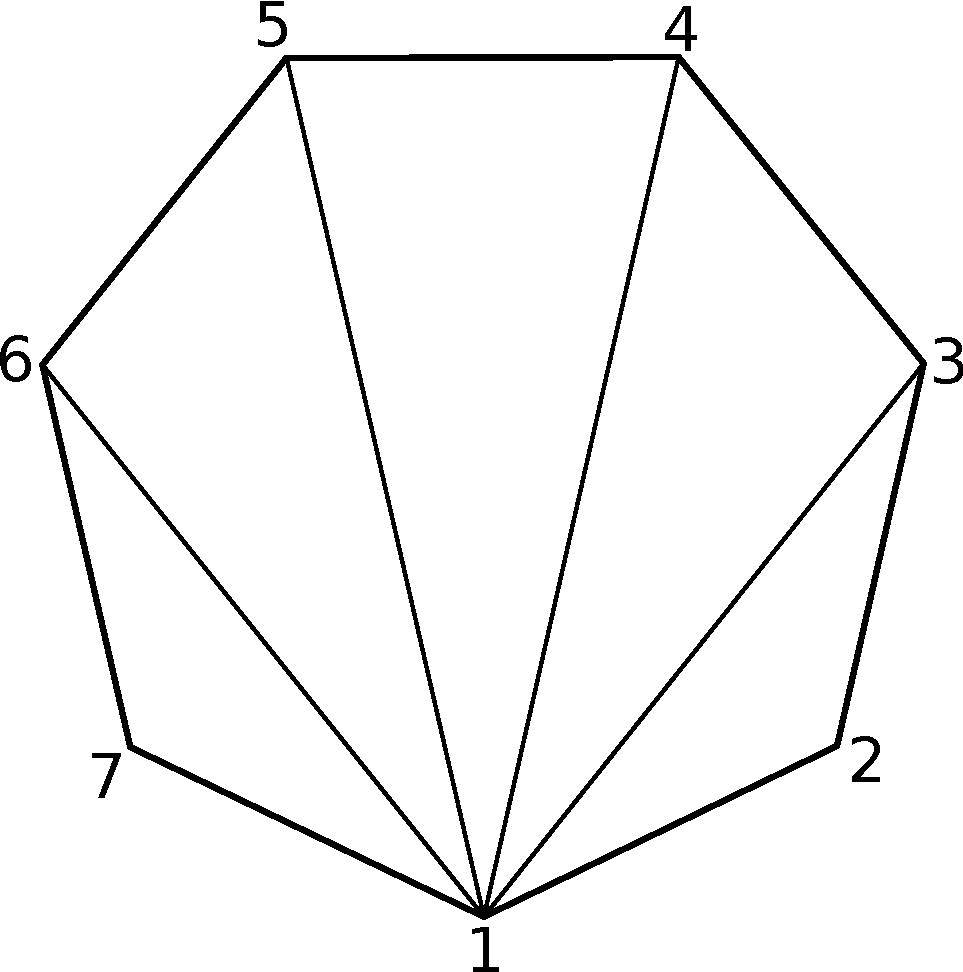
\includegraphics[width=0.3\textwidth]{fig/TriangleFan.pdf}
	\caption[OBJ Polygon to Triangle Fan]{Polygon represented through a Triangle Fan\protect}
	\label{fig:TriangleFan}
\end{figure}

A group determines what faces are combined in order to make a component of the larger object. The "usemtl" tags tells what material should be used on the faces and that material is used until the next tag appears. The actual materials are defined in an MTL file, which works similarly to an OBJ, just with different tags and values. Some of the more important entries can be seen in Table \ref{tab:MTLTypes}. This MTL file of course also needs to be shared to every client. The values themselves are saved in a 2D array where every row defines one material and every column a specific value. 

\begin{table}[htbp]
	\centering 
	\scalebox{0.889}{
		\begin{tabular}{lll}
			\toprule \textbf{Tag} & \textbf{Example Value} & \textbf{Definition} \\
			\bottomrule
			newmtl & White & Defines a new Material\\
			Ka & 1.0 1.0 1.0 & Ambient colour\\
			Kd & 0.0 0.0 0.0 &  Diffuse Colour\\
			Ks & 1.0 1.0 1.0& Specular Colour\\
			d & 0.5 & Transparency\\
			
			\bottomrule
	\end{tabular}}
	\caption[MTL Types]{Relevant types in MTL format}
	\label{tab:MTLTypes}
\end{table}

Due to all of this, these values need to be combined and saved in an array where every array entry represents one group. The group consists of the face values and marks where materials need to be switched.\\
The only major problem with OBJ is the fact that the coordinates don't have units, meaning they can't be scaled to properly represent the designed size. Instead everything is scaled with same factor so that at least the scales between objects made in the same scene stay the same. Also the created objects can later be scaled by users to better resemble the desired size.

\subsubsection{STL}
STL is a file format native to the CAD software created by 3D Systems in 1987\cite{}. The format has gained a lot of support in many different software packages, especially for 3D printing software where it is one of the default formats. STL files only describe the surface geometry of a three-dimensional object with out any additional information about colours, materials or groups. The geometry is described in raw, unstructured triangles defined by a normal and 3 vertices. The way a triangle is defined in the file is shown in Figure \ref{fig:STLFormat}. 
\begin{figure}[htpb]
	\centering
	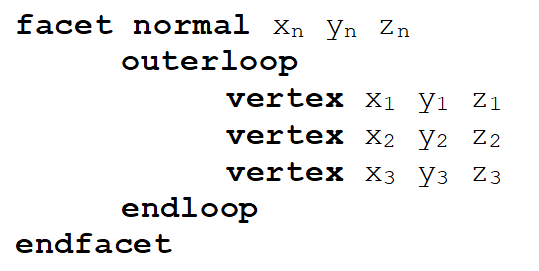
\includegraphics[width=0.35\textwidth]{fig/STLFormat.png}
	\caption[STL Triangle facet]{A triangle facet represented in STL\protect}
	\label{fig:STLFormat}
\end{figure}

While the structure suggests that multiple possibilities are possible for loops, the facets can only be triangles. In order to represent a full model the triangles are simply listed one after the other. In order to parse it, the vertices and normals are saved in arrays and faces are generated to point what vertices make up the triangles. This is important for generating the mesh later. While it is a simpler format compared to OBJ, it is excellent when only the shape is relevant. It does unfortunately suffer from the same scaling problems as OBJ and that is handled in the same way as well.\\
Overall with these two formats the majority of the most common and well-known CAD formats are covered. Ideally more formats would be covered and specific parsers for every format would be written to get the most accurate results but for the limitations of this project, this is a very practical solution.

%%%%%%%%%%%%%%%%%%%%%%%%%%%%%%%%%%%%%%%%%%%%%%%%%%%%%%%%%%%%%%%%%%%%%%%%%%%%%%%%%%%%%%%%%%%%%%%%%%%%%%%%%%%%%%
\section{Runtime Mesh Generation}

After the files have been parsed and the needed data was extracted, the actual process of creating a new 3D object starts. For that, a way to tell Unreal to generate a mesh is required and Unreal does in fact support such a feature in the form of so called Procedural Mesh Components(PMC). These components can be created in runtime by giving them the required mesh data and letting them generate themselves. In the first phases of this project it was explored as to how viable using these components were. Getting it to function took a bit of work, mostly due to Unreal Engines generally bad documentation, but the first results with small object were quite promising. Unfortunately the problems started to arise with larger objects where the performance would drop significantly or the Unreal editor would simply crash. The reason for this lies within the procedural mesh components themselves. As the name implies, these components are supposed to be generated by some form of procedure which generally won't create nearly as many vertices as a large CAD file can. On top of that the underlying architecture for a real procedural system for expensive geometrical operations would be quite different to that of a runtime gameplay framework \cite{}. So even though it is designed for a quite similar purpose, it is different enough that it couldn't be used.\\
Due to this a different method of getting Unreal to generate meshes had to be found and during this time a very important question came up. Doesn't Unreal technically already support runtime mesh generation? Let's say, as an example, there was an Actor that had some sort of static mesh attached to it. Unreal could spawn in this new Actor without a problem. So why can't it also create such an Actor from data parsed from a file?\\
A definitive answer for that question couldn't be found but through some research a few speculations can be made. The biggest reason for this probably stems from the main purpose of Unreal Engine. Unreal has always and will probably always be a video game engine. As such it is designed and optimized for use cases that happen in video games.

% no use in games
% hardware not good enough especially not for CAD files which are generally one of the most demanding
% not until recently was there a need for this
% this can espcially be seen with the fact that datasmith itself is didn't come to be until 2016
% but there was still very much a need for it and RMC came to be it's a library 
%While ideally for this a library wouldn't need to be used, it is unrealistic that in the scope of this project a solution could be designed that works better than a software which has been in development for more than 5 years and had more than 40 people contribute to it.

\subsubsection{Generating a CAD Model}

Before a model can be inserted at
The first step to inserting a model into a scene at runtime is spawning in an Actor to which the newly generated components can be attached to. Spawning in an Actor is quite simple, a Blueprint function for that is built into Unreal already. The only two parameters that are required is the class of the Actor and the location where it should be spawned.

%%%%%%%%%%%%%%%%%%%%%%%%%%%%%%%%%%%%%%%%%%%%%%%%%%%%%%%%%%%%%%%%%%%%%%%%%%%%%%%%%%%%%%%%%%%%%%%%%%%%%%%%%%%%%%

\section{Object Interaction}\label{chp:ObjectInteraction}
While being able to generate 3D models is quite handy, it would be severely limited if it just stood in a place and the users had no way of doing anything with the model. That is why it is important to take a look at how it possible to interact with these objects. There are many ways in which this can be done so the presented solutions are just what was implemented in CRP to demonstrate some of the more basic interactions that can probably be useful for most projects. 


\subsection{Grabbing and Translating}

One of the most basic but also important interactions a user can have with an object is grabbing it and moving it around in the scene.

\subsection{Grabbing Individual Components}

As already mentioned, the model generally consists of many smaller components and while it is great to be able to interact with it as a whole, it could be a lot more useful if a user could choose to interact with every component individually.
%hovering

\subsection{Scaling and Rotating}

\subsection{Duplication, Expansion and Deletion}



